\section{Introduction}
 A battery is filled with reagents, connecting a battery to the circuit causes chemical reaction. During the reaction there is a an electron flow from anode(negatively charged plate) to cathode(positively charged plate) which causes the circuit to operate. As the chemical reactions inside the battery uses up limited reagents, the battery performance will drop.\citep{schmidt2018batteries} The battery that was used for this project is manufactured by Energizer Alkaline 9V battery (\autoref{fig:battery}). The battery is considered "dead" if its voltage drops to 4.8V.\citep{batterydatasheet}\\
\begin{figure}[h!]
\centering
\begin{subfigure}{.3\textwidth}
  \centering
  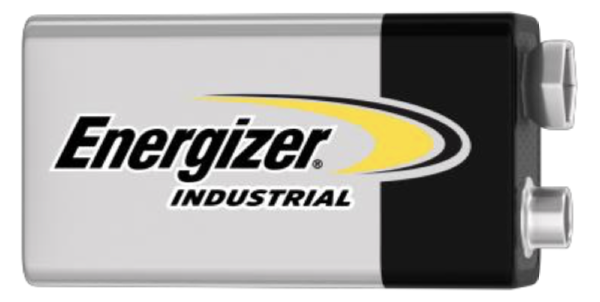
\includegraphics[width=\textwidth]{battery1.png}
  \caption{Visual of A Battery}
  \label{fig:sub1}
\end{subfigure}%
\hspace{3cm}
\begin{subfigure}{.3\textwidth}
  \centering
  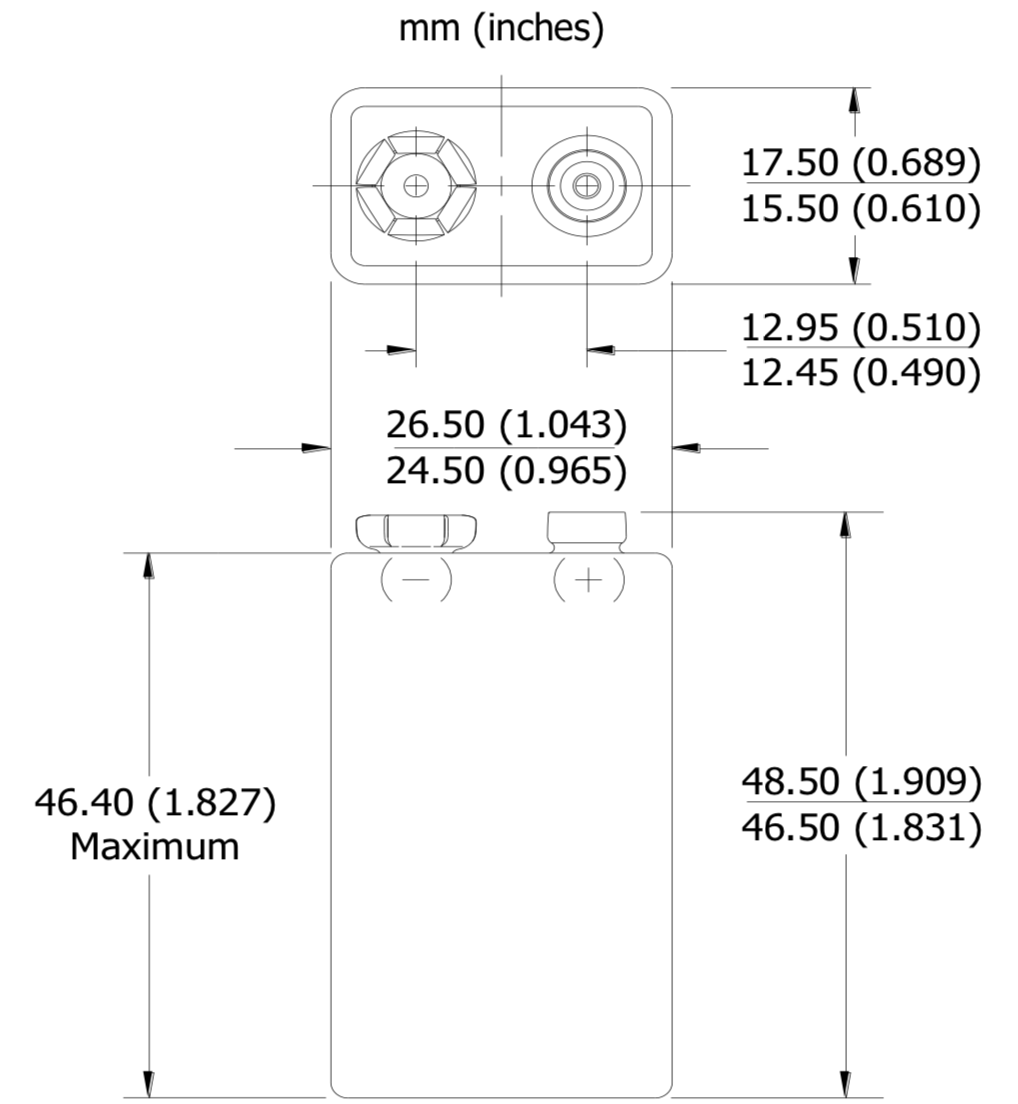
\includegraphics[width=\textwidth]{battery2.png}
  \caption{Dimensions of A Battery}
  \label{fig:sub2}
\end{subfigure}
\caption{Representation of A Battery Utilized}
\label{fig:battery}
\end{figure}
To record the data of the battery, it is going to be connected to Raspberry Pi using ADC0831 chip and voltage divider. Raspberry Pi is a minicomputer that capable of connecting and talking to microcontroller chips to record and manipulate data via programming languages. Refer \autoref{fig:pinout} for Raspberry Pi's pinout. \\
The ADC0831 is a chip that was designed to take data for you with minimum effort, because the process is automated. The chip is a 8-bit serial input/output analog/digital converter chip. Basically, it converts an analog measurement to binary, so it can interact with you through computer.\citep{adcdatasheet} See \autoref{fig:chip} for chip. \newpage
\begin{figure}[ht]
\centering
\begin{subfigure}{.27\textwidth}
  \centering
  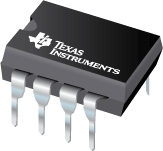
\includegraphics[width=\textwidth]{ADC0831-N.jpg}
  \caption{Visual of ADC0831 chip}
  \label{fig:sub3}
\end{subfigure}%
\hspace{3cm}
\begin{subfigure}{.3\textwidth}
  \centering
  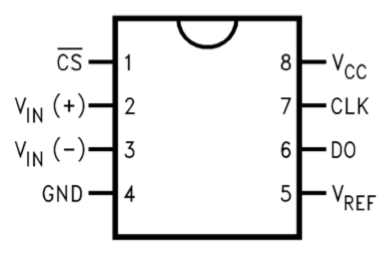
\includegraphics[width=\textwidth]{adc0831.png}
  \caption{Pin Map}
  \label{fig:sub4}
\end{subfigure}
\caption{ADC0831 Microcontroller Chip}
\label{fig:chip}
\end{figure}
\noindent
The voltage divider allows us to decrease input voltage to desired output voltage value by varying resistors in circuit shown in  \autoref{fig:voltdivintro}.
\begin{figure}[h]
\centering
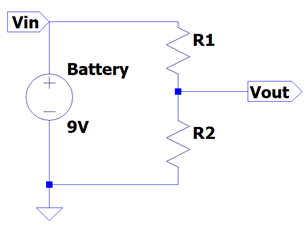
\includegraphics[width=0.4\textwidth]{voltdiv.png}
\caption{The Voltage Divider}
\label{fig:voltdivintro}
\end{figure}\newline
From the  \autoref{fig:voltdivintro} we can see the current flow is:
\begin{equation}
    {I} = \frac{{V_{in}}}{R_1 + R_2}
    \label{eq:current}
\end{equation}{}
The voltage across the second resistor is $V_{out} = I * R_2$, which yields
\begin{equation}
   \frac{{V_{out}}} {R_2} = \frac{{V_{in}}}{R_1 + R_2}
    \label{eq:V_out}
\end{equation}{}
Rearranging term in \autoref{eq:V_out}, it can be shown:
\begin{equation}
    \frac{V_{out}}{V_{in}} = \frac{R_2}{R_1 + R_2}
    \label{eq:voltdiv}
\end{equation}{}
This voltage divider relationship allows output voltage to be any desired value.\citep{meyer}